% block_foldy_lax.tex — Block-Preconditioned Foldy-Lax Solver
% Compile with: lualatex block_foldy_lax.tex
\documentclass[11pt,a4paper]{article}

\usepackage{fontspec}
\setmainfont{Latin Modern Roman}
\setmonofont{Latin Modern Mono}

\usepackage{amsmath,amssymb,amsthm}
\usepackage{mathtools}
\usepackage{bm}
\usepackage{booktabs}
\usepackage[svgnames]{xcolor}
\usepackage{geometry}
\geometry{margin=2.5cm}

\usepackage{hyperref}
\hypersetup{
  colorlinks=true,
  linkcolor=DarkBlue,
  citecolor=DarkBlue,
  urlcolor=DarkBlue,
}

\usepackage{enumitem}
\usepackage{fancyhdr}
\pagestyle{fancy}
\fancyhf{}
\fancyhead[L]{\small Block-Preconditioned Foldy-Lax Solver for Layered Elastic Media}
\fancyhead[R]{\small\thepage}
\renewcommand{\headrulewidth}{0.4pt}

% TikZ and pgfplots
\usepackage{tikz}
\usepackage{pgfplots}
\pgfplotsset{compat=1.18}
\usepgfplotslibrary{groupplots}
\usetikzlibrary{arrows.meta,positioning,shapes.geometric,patterns,calc}

% Notation shortcuts
\newcommand{\dd}{\mathrm{d}}
\newcommand{\ppd}[2]{\frac{\partial #1}{\partial #2}}

\theoremstyle{plain}
\newtheorem{proposition}{Proposition}
\theoremstyle{remark}
\newtheorem{remark}{Remark}

\title{%
  Block-Preconditioned Foldy-Lax Solver for Layered Elastic Media\\[6pt]
  \large Space-Filling Cubic Heterogeneities in a Marine Sedimentary Model%
}
\author{}
\date{}

\begin{document}
\maketitle
\thispagestyle{fancy}

\begin{abstract}
We present a block-preconditioned Foldy-Lax solver for elastic multiple
scattering from space-filling cubic heterogeneities embedded in a layered
marine sedimentary model.  The solver operates in a coupled 9-component
displacement-strain basis and exploits the depth-layer structure of the
scatterer array: intra-layer interactions ($\Delta z = 0$) are evaluated
via 2D FFT convolution, while inter-layer coupling ($\Delta z \ne 0$) is
handled by an outer GMRES iteration.  A block-Jacobi preconditioner
solves each z-layer independently.  The solver is validated against a
dense reference solve with relative errors below $10^{-7}$, matching the
GMRES convergence tolerance.  A slab thickness sweep reveals monotonic
growth of the per-cube composite T-matrix norm with the number of
z-layers, quantifying interlayer vertical multiple scattering.
The dressed T-matrix, which captures intra-layer horizontal multiple
scattering via a lattice self-energy, is compared against the bare T
in the Riccati interlayer reflectivity solver.
\end{abstract}

%=============================================================================
\section{Introduction}\label{sec:intro}
%=============================================================================

Elastic wave scattering from heterogeneous inclusions in marine sediments
is a fundamental problem in exploration seismology.  When the scatterers
form a dense lattice of cubic heterogeneities filling a sedimentary layer,
the classical Foldy-Lax multiple scattering equation governs the exciting
field at each scatterer:
\begin{equation}\label{eq:foldy-lax}
  \bigl(\mathbf{I} - \mathbf{G} \cdot \mathbf{T}\bigr)\,\bm{\psi}
  = \bm{\psi}_{\mathrm{inc}},
\end{equation}
where $\mathbf{G}$ is the free-space elastic Green's tensor,
$\mathbf{T}$ is the block-diagonal T-matrix operator (encoding each
cube's scattering response in the 9-component displacement-strain basis),
and $\bm{\psi}_{\mathrm{inc}}$ is the incident field.

The key physical insight underlying the block-preconditioned solver is
the separation of length scales in layered media: intra-layer
propagators ($\Delta z = 0$) exhibit slow algebraic decay
$\sim 1/k_H$ in the horizontal wavenumber, while inter-layer propagators
($\Delta z \ne 0$) decay exponentially as $\sim\exp(-\kappa|\Delta z|)$,
where $\kappa$ is the evanescent vertical wavenumber.  This separation
motivates a two-level solve: fast 2D FFT convolution within each
z-layer and an outer GMRES iteration over the inter-layer coupling.

Section~\ref{sec:model} describes the marine layer model.
Section~\ref{sec:heterogeneity} defines the heterogeneity parameters and
the dressed T-matrix.  Section~\ref{sec:solver} presents the
block-preconditioned solver algorithm.
Section~\ref{sec:validation} validates the solver against a dense
reference.  Section~\ref{sec:thickness} examines the effect of slab
thickness on the composite T-matrix.  Section~\ref{sec:reflectivity}
compares bare and dressed T-matrices in the Riccati interlayer
reflectivity solver.  Section~\ref{sec:conclusions} summarises the
findings.

%=============================================================================
\section{Marine Layer Model}\label{sec:model}
%=============================================================================

The background medium is a four-layer marine sedimentary model:
an acoustic ocean overlying two elastic sediment layers and a basement
half-space.  Heterogeneous cubic inclusions are embedded in the target
sediment layer (between interfaces~1 and~2).

\begin{table}[ht]
\centering
\renewcommand{\arraystretch}{1.2}
\caption{Marine layer model parameters.  Velocities in km/s, densities
in g/cm$^3$, thicknesses in km.}
\label{tab:model}
\begin{tabular}{clcccccc}
  \toprule
  \textbf{Layer} & \textbf{Description} & $\alpha$ & $\beta$
    & $\rho$ & $h$ & $Q_\alpha$ & $Q_\beta$ \\
  \midrule
  0 & Ocean           & 1.5 & 0.0 & 1.0 & 1.0    & 20\,000 & $\infty$ \\
  1 & Soft sediment   & 2.0 & 0.8 & 1.8 & 0.5    & 200     & 200 \\
  2 & Target sediment & 3.0 & 1.5 & 2.5 & 1.0    & 200     & 200 \\
  3 & Basement        & 5.0 & 2.8 & 3.0 & $\infty$ & 200   & 200 \\
  \bottomrule
\end{tabular}
\end{table}

\begin{figure}[ht]
\centering
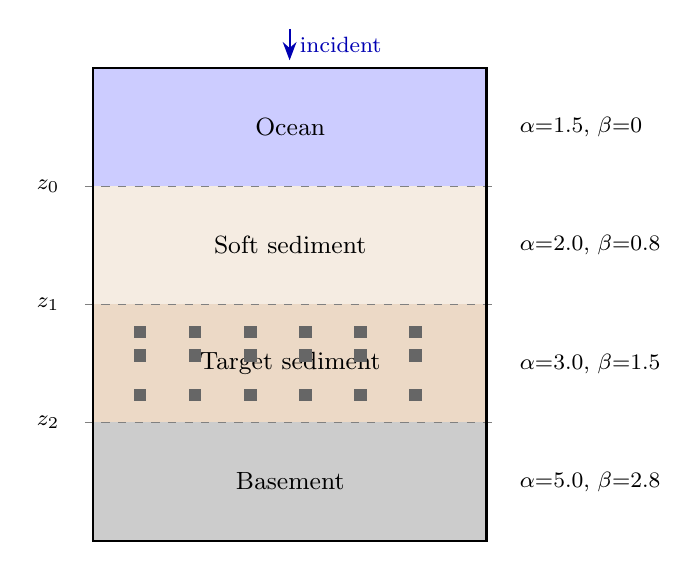
\begin{tikzpicture}[
  layer/.style={minimum width=5cm, minimum height=1.5cm,
    text=black, font=\small, align=center},
  iface/.style={font=\footnotesize},
  param/.style={font=\footnotesize, text=black},
  >=Stealth,
]
  % Ocean
  \node[layer, fill=blue!20, anchor=south west] (L0) at (0,4.5)
    {Ocean};
  % Soft sediment
  \node[layer, fill=brown!15, anchor=south west] (L1) at (0,3.0)
    {Soft sediment};
  % Target (with cubes)
  \node[layer, fill=brown!30, anchor=south west] (L2) at (0,1.5)
    {Target sediment};
  % Basement
  \node[layer, fill=gray!40, anchor=south west] (L3) at (0,0)
    {Basement};

  % Small cubes in target layer
  \foreach \x in {0.6,1.3,2.0,2.7,3.4,4.1} {
    \foreach \y in {1.85,2.35,2.65} {
      \fill[black!60] (\x-0.08,\y-0.08) rectangle (\x+0.08,\y+0.08);
    }
  }

  % Interface labels (left)
  \node[iface, anchor=east] at (-0.3,4.5) {$z_0$};
  \node[iface, anchor=east] at (-0.3,3.0) {$z_1$};
  \node[iface, anchor=east] at (-0.3,1.5) {$z_2$};

  % Dashed interface lines
  \draw[dashed, gray] (-0.1,4.5) -- (5.1,4.5);
  \draw[dashed, gray] (-0.1,3.0) -- (5.1,3.0);
  \draw[dashed, gray] (-0.1,1.5) -- (5.1,1.5);

  % Velocity labels (right)
  \node[param, anchor=west] at (5.3,5.25) {$\alpha{=}1.5$, $\beta{=}0$};
  \node[param, anchor=west] at (5.3,3.75) {$\alpha{=}2.0$, $\beta{=}0.8$};
  \node[param, anchor=west] at (5.3,2.25) {$\alpha{=}3.0$, $\beta{=}1.5$};
  \node[param, anchor=west] at (5.3,0.75) {$\alpha{=}5.0$, $\beta{=}2.8$};

  % Incident wave arrow
  \draw[->, thick, blue!70!black] (2.5,6.5) -- (2.5,6.1)
    node[midway, right, font=\footnotesize] {incident};

  % Outer box
  \draw[thick] (0,0) rectangle (5,6);
\end{tikzpicture}
\caption{Marine sedimentary model.  Four layers with cubic
heterogeneities (small squares) embedded in the target sediment layer.
Velocities in km/s.}
\label{fig:model}
\end{figure}

%=============================================================================
\section{Heterogeneity Parameters}\label{sec:heterogeneity}
%=============================================================================

The heterogeneous inclusions are space-filling cubes with half-width
$a = 10$~m and lattice spacing $d = 2a = 20$~m (cubes touching).  The
areal number density is $n = 1/d^2 = 0.0025$~m$^{-2}$.  The reference
medium for the cube T-matrix computation is the target sediment
($\alpha = 3000$~m/s, $\beta = 1500$~m/s, $\rho = 2500$~kg/m$^3$).

We consider two contrasts: a \emph{moderate} contrast for the block
solver validation (ensuring rapid GMRES convergence), and a \emph{hard}
contrast for the reflectivity comparison.  At the test frequency
$f = 15$~Hz, $ka \approx 0.31$.

\begin{table}[ht]
\centering
\renewcommand{\arraystretch}{1.2}
\caption{Material contrast parameters (SI units) and dressed T-matrix
corrections at $f = 15$~Hz with $n_{\mathrm{rings}} = 20$.}
\label{tab:contrast}
\begin{tabular}{lcccc}
  \toprule
  \textbf{Contrast} & $\Delta\lambda$ (Pa) & $\Delta\mu$ (Pa)
    & $\Delta\rho$ (kg/m$^3$) & Dressed correction \\
  \midrule
  Moderate & $3.0 \times 10^9$  & $1.5 \times 10^9$  & 100  & 16.2\% \\
  Hard     & $2.14 \times 10^{10}$ & $2.18 \times 10^{10}$ & 1000 & 275\% \\
  \bottomrule
\end{tabular}
\end{table}

The \emph{dressed} T-matrix incorporates the lattice self-energy from
surrounding scatterers in the same horizontal layer:
\begin{equation}\label{eq:dressed-T}
  \mathbf{T}_{\mathrm{dressed}}
  = \mathbf{T}_{\mathrm{bare}}
    \bigl(\mathbf{I}
    - \mathbf{\Sigma}_{\mathrm{self}} \cdot
    \mathbf{T}_{\mathrm{bare}}\bigr)^{-1},
\end{equation}
where $\mathbf{\Sigma}_{\mathrm{self}}$ is the lattice Green's function
sum over $n_{\mathrm{rings}}$ rings of neighbours.  The dressed T
captures intra-layer (horizontal) multiple scattering while the bare T
ignores it entirely.  For the hard contrast, the dressed correction
exceeds 275\%, indicating that the bare T is a poor approximation for
individual scatterer response in a dense lattice.

%=============================================================================
\section{Block-Preconditioned Solver}\label{sec:solver}
%=============================================================================

The solver exploits the regular lattice geometry of an $M \times M
\times N_z$ array of cubes to decompose the Foldy-Lax system by
depth layer.

\subsection{Layer decomposition}

Cubes are grouped by z-index into $N_z$ horizontal layers, each
containing $M^2$ cubes.  The decomposition induces a block structure
on the system matrix $(\mathbf{I} - \mathbf{G}\cdot\mathbf{T})$:
intra-layer blocks (diagonal) correspond to $\Delta z = 0$, while
inter-layer blocks (off-diagonal) correspond to $\Delta z \ne 0$.

\begin{figure}[ht]
\centering
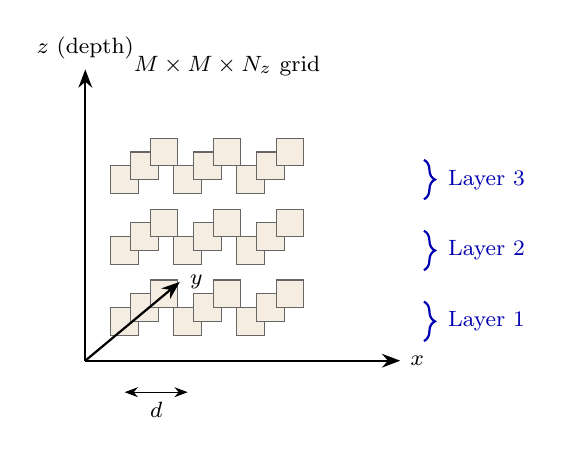
\begin{tikzpicture}[
  >=Stealth,
  cube/.style={draw=black!60, fill=brown!15, minimum size=0.35cm},
]
  % 3D perspective of cube lattice
  \def\dx{0.8}  % x spacing
  \def\dy{0.5}  % y spacing (perspective)
  \def\dz{0.9}  % z spacing

  % Draw cubes in 3x3x3 grid
  \foreach \iz in {0,1,2} {
    \foreach \ix in {0,1,2} {
      \foreach \iy in {0,1,2} {
        \pgfmathsetmacro{\px}{\ix*\dx + \iy*\dy*0.5}
        \pgfmathsetmacro{\py}{\iz*\dz + \iy*\dy*0.35}
        \node[cube] at (\px, \py) {};
      }
    }
  }

  % Axis arrows
  \draw[->, thick] (-0.5,-0.5) -- (3.5,-0.5)
    node[right, font=\footnotesize] {$x$};
  \draw[->, thick] (-0.5,-0.5) -- (-0.5,3.2)
    node[above, font=\footnotesize] {$z$ (depth)};
  \draw[->, thick] (-0.5,-0.5) -- (0.7,0.5)
    node[right, font=\footnotesize] {$y$};

  % Dimension labels
  \draw[<->, thin] (0,-0.9) -- (\dx,-0.9)
    node[midway, below, font=\footnotesize] {$d$};

  % Layer brackets
  \draw[decorate, decoration={brace, amplitude=4pt, mirror},
    thick, blue!70!black]
    (3.8,0-0.25) -- (3.8,0+0.25)
    node[midway, right=5pt, font=\footnotesize] {Layer 1};
  \draw[decorate, decoration={brace, amplitude=4pt, mirror},
    thick, blue!70!black]
    (3.8,\dz-0.25) -- (3.8,\dz+0.25)
    node[midway, right=5pt, font=\footnotesize] {Layer 2};
  \draw[decorate, decoration={brace, amplitude=4pt, mirror},
    thick, blue!70!black]
    (3.8,2*\dz-0.25) -- (3.8,2*\dz+0.25)
    node[midway, right=5pt, font=\footnotesize] {Layer 3};

  % Label M and Nz
  \node[font=\footnotesize, anchor=south] at (1.3,3.0)
    {$M \times M \times N_z$ grid};
\end{tikzpicture}
\caption{Cube lattice geometry showing $M \times M \times N_z$ regular
grid with spacing $d = 2a$.  Cubes within each z-layer (highlighted by
brackets) interact via 2D FFT convolution; inter-layer coupling is
handled by the outer GMRES.}
\label{fig:lattice}
\end{figure}

\subsection{Intra-layer 2D FFT kernel}

For cubes within the same z-layer, the Green's function depends only on
the horizontal separation $(\Delta x \cdot d,\; \Delta y \cdot d)$.
The interaction kernel is constructed as:
\begin{equation}\label{eq:intra-kernel}
  K_{\mathrm{intra}}[\Delta x, \Delta y]
  = -\mathbf{P}_{9\times 9}\bigl(\mathbf{0},\; \Delta x \cdot d,\;
    \Delta y \cdot d\bigr) \cdot \mathbf{T}_{\mathrm{loc}},
\end{equation}
where $\mathbf{P}_{9\times 9}$ is the coupled displacement-strain
propagator and $\mathbf{T}_{\mathrm{loc}}$ is the local T-matrix.  The
kernel is embedded in a $2M \times 2M$ circular convolution grid and
diagonalised via a 2D FFT.  The intra-layer matrix-vector product then
costs $O(M^2 \log M)$ per column.

\subsection{Inter-layer kernels}

For cubes in different z-layers separated by $\Delta z \ne 0$, the
same propagator structure applies with the additional vertical offset.
Kernels are precomputed and cached by $|\Delta z|$, exploiting the
translational symmetry of each layer pair.

\subsection{Layered matrix-vector product}

The full matrix-vector product $(\mathbf{I} - \mathbf{G}\cdot
\mathbf{T})\mathbf{w}$ is computed as:
\begin{enumerate}[nosep]
  \item For each z-layer pair $(l, l')$: apply the 2D FFT convolution
    kernel (intra-layer if $l = l'$, inter-layer otherwise).
  \item Sum contributions across all source layers to obtain the
    residual for each target layer.
\end{enumerate}

\subsection{Block-Jacobi preconditioner}

The preconditioner inverts each intra-layer diagonal block independently
via a per-layer GMRES solve with the same 2D FFT kernel.  This
preconditioner is effective when the inter-layer coupling is weaker
than the intra-layer interaction, which holds for the exponentially
decaying inter-layer Green's function.

\begin{figure}[ht]
\centering
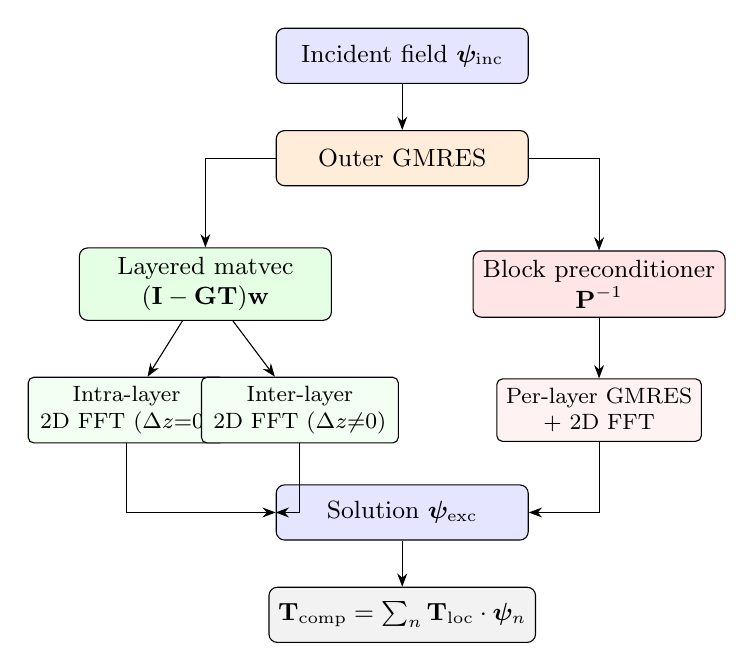
\begin{tikzpicture}[
  >=Stealth,
  box/.style={draw, rounded corners=3pt, minimum width=3.2cm,
    minimum height=0.7cm, align=center, font=\small},
  smallbox/.style={draw, rounded corners=2pt, minimum width=2.5cm,
    minimum height=0.55cm, align=center, font=\footnotesize},
]
  % Top: incident field
  \node[box, fill=blue!10] (inc) at (0,5.5)
    {Incident field $\bm{\psi}_{\mathrm{inc}}$};

  % Outer GMRES
  \node[box, fill=orange!15] (gmres) at (0,4.2)
    {Outer GMRES};

  % Matvec
  \node[box, fill=green!10] (mv) at (-2.5,2.6)
    {Layered matvec\\$(\mathbf{I}-\mathbf{G}\mathbf{T})\mathbf{w}$};

  % Preconditioner
  \node[box, fill=red!10] (prec) at (2.5,2.6)
    {Block preconditioner\\$\mathbf{P}^{-1}$};

  % Sub-boxes
  \node[smallbox, fill=green!5] (intra) at (-3.5,1.0)
    {Intra-layer\\2D FFT ($\Delta z{=}0$)};
  \node[smallbox, fill=green!5] (inter) at (-1.3,1.0)
    {Inter-layer\\2D FFT ($\Delta z{\ne}0$)};
  \node[smallbox, fill=red!5] (perlayer) at (2.5,1.0)
    {Per-layer GMRES\\+ 2D FFT};

  % Output
  \node[box, fill=blue!10] (sol) at (0,-0.3)
    {Solution $\bm{\psi}_{\mathrm{exc}}$};

  % T_comp
  \node[box, fill=gray!10] (tcomp) at (0,-1.6)
    {$\mathbf{T}_{\mathrm{comp}}
     = \sum_n \mathbf{T}_{\mathrm{loc}} \cdot \bm{\psi}_n$};

  % Arrows
  \draw[->] (inc) -- (gmres);
  \draw[->] (gmres) -| (mv);
  \draw[->] (gmres) -| (prec);
  \draw[->] (mv) -- (intra);
  \draw[->] (mv) -- (inter);
  \draw[->] (prec) -- (perlayer);
  \draw[->] (intra) |- (sol);
  \draw[->] (inter) |- (sol);
  \draw[->] (perlayer) |- (sol);
  \draw[->] (sol) -- (tcomp);
\end{tikzpicture}
\caption{Algorithm flowchart.  The outer GMRES calls the layered
matrix-vector product (intra-layer and inter-layer 2D FFT convolutions)
and the block-Jacobi preconditioner (independent per-layer GMRES).  The
composite T-matrix is assembled from the converged exciting field.}
\label{fig:flowchart}
\end{figure}

%=============================================================================
\section{Numerical Validation}\label{sec:validation}
%=============================================================================

The block solver is validated against a dense reference solve that
explicitly constructs the full $(\mathbf{I} - \mathbf{G}\cdot
\mathbf{T})$ matrix and solves via direct linear algebra.  Both methods
compute the composite T-matrix $\mathbf{T}_{\mathrm{comp}} = \sum_n
\mathbf{T}_{\mathrm{loc}} \cdot \bm{\psi}_n^{\mathrm{exc}}$.  The test
uses the moderate contrast at $f = 15$~Hz.

\begin{table}[ht]
\centering
\renewcommand{\arraystretch}{1.2}
\caption{Block solver vs.\ dense reference (moderate contrast,
$f = 15$~Hz).  All configurations converge with 9 GMRES iterations
per right-hand-side column.}
\label{tab:validation}
\begin{tabular}{rrrrl}
  \toprule
  $M$ & $N_z$ & $n_C$ & Iterations & Relative error \\
  \midrule
  3 & 1 &  9 & 9 & $2.38 \times 10^{-8}$ \\
  5 & 1 & 25 & 9 & $3.35 \times 10^{-7}$ \\
  3 & 2 & 18 & 9 & $2.76 \times 10^{-9}$ \\
  5 & 2 & 50 & 9 & $1.92 \times 10^{-7}$ \\
  3 & 3 & 27 & 9 & $1.76 \times 10^{-9}$ \\
  \bottomrule
\end{tabular}
\end{table}

The maximum relative error across all configurations is
$3.35 \times 10^{-7}$, matching the GMRES convergence tolerance of
$10^{-8}$.  The block solver reproduces the dense reference to the
expected numerical precision, confirming that the 2D FFT convolution
correctly implements the Foldy-Lax system.

%=============================================================================
\section{Slab Thickness Effect}\label{sec:thickness}
%=============================================================================

For $N_z > 1$, the Foldy-Lax solver captures interlayer (vertical)
multiple scattering between cube layers within the heterogeneous slab.
We examine $\|\mathbf{T}_{\mathrm{comp}} / n_C\|$ as a function of
$N_z$ for a fixed $M = 5$ grid with moderate contrast.

\begin{figure}[ht]
\centering
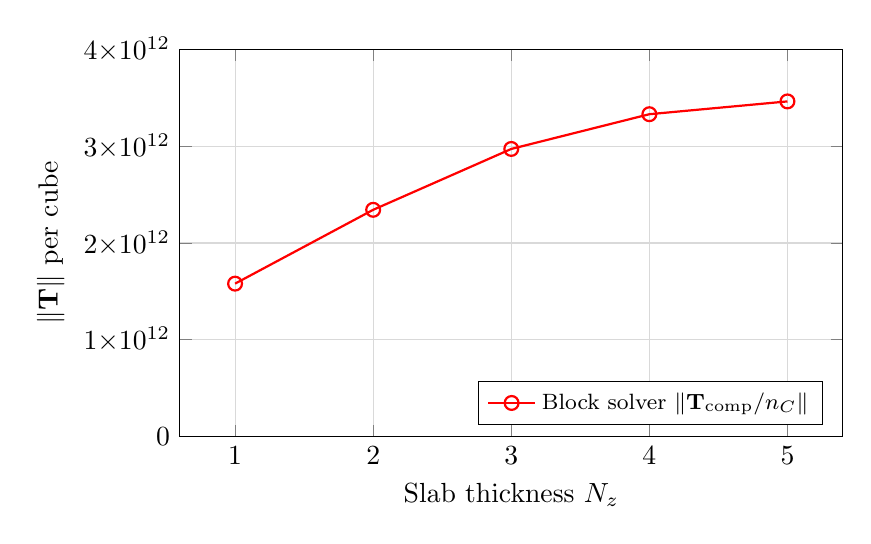
\begin{tikzpicture}
\begin{axis}[
  width=10cm, height=6.5cm,
  xlabel={Slab thickness $N_z$},
  ylabel={$\|\mathbf{T}\|$ per cube},
  xtick={1,2,3,4,5},
  ymin=0, ymax=4e12,
  scaled y ticks=false,
  ytick={0,1e12,2e12,3e12,4e12},
  yticklabels={$0$,$1{\times}10^{12}$,$2{\times}10^{12}$,
    $3{\times}10^{12}$,$4{\times}10^{12}$},
  legend pos=south east,
  legend style={font=\footnotesize},
  grid=major,
  grid style={gray!30},
]
\addplot[red, mark=o, thick, mark size=2.5pt] coordinates {
  (1, 1.5798e12)
  (2, 2.3423e12)
  (3, 2.9709e12)
  (4, 3.3297e12)
  (5, 3.4619e12)
};
\addlegendentry{Block solver $\|\mathbf{T}_{\mathrm{comp}}/n_C\|$}
\end{axis}
\end{tikzpicture}
\caption{Per-cube composite T-matrix norm vs.\ slab thickness ($M = 5$,
moderate contrast, $ka \approx 0.31$).  The monotonic increase with
$N_z$ quantifies the additional interlayer (vertical) multiple
scattering captured by the Foldy-Lax solve.  The norm at $N_z = 1$
includes only horizontal coupling within the $5 \times 5$ grid.}
\label{fig:thickness}
\end{figure}

The per-cube norm increases monotonically from $1.58 \times 10^{12}$ at
$N_z = 1$ to $3.46 \times 10^{12}$ at $N_z = 5$ --- a factor of 2.2.
The $N_z = 1$ value represents horizontal-only MS within the finite
$5 \times 5$ grid, while each additional z-layer adds vertical coupling
channels.  The growth rate decreases with $N_z$, approaching saturation
as the slab thickness exceeds the evanescent decay length of the
inter-layer Green's function.

The dressed T-matrix norm for the infinite horizontal plane
($n_{\mathrm{rings}} = 20$) is $9.80 \times 10^{13}$ --- roughly 60
times larger than the $N_z = 1$ block solver result.  This gap reflects
the finite grid size ($M = 5$): the block solver sums over only
$5 \times 5 = 25$ cubes per layer, while the dressed T sums over
approximately $1{,}260$ neighbours in 20 rings.

%=============================================================================
\section{Ocean-Bottom Reflectivity}\label{sec:reflectivity}
%=============================================================================

The bare and dressed T-matrices (hard contrast) are fed into the
Riccati interlayer multiple scattering solver as scatterers at
interfaces~1 and~2, and ocean-bottom reflectivity is computed as a
function of frequency at horizontal wavenumber $k_H = 3.0$~km$^{-1}$.

\begin{figure}[ht]
\centering
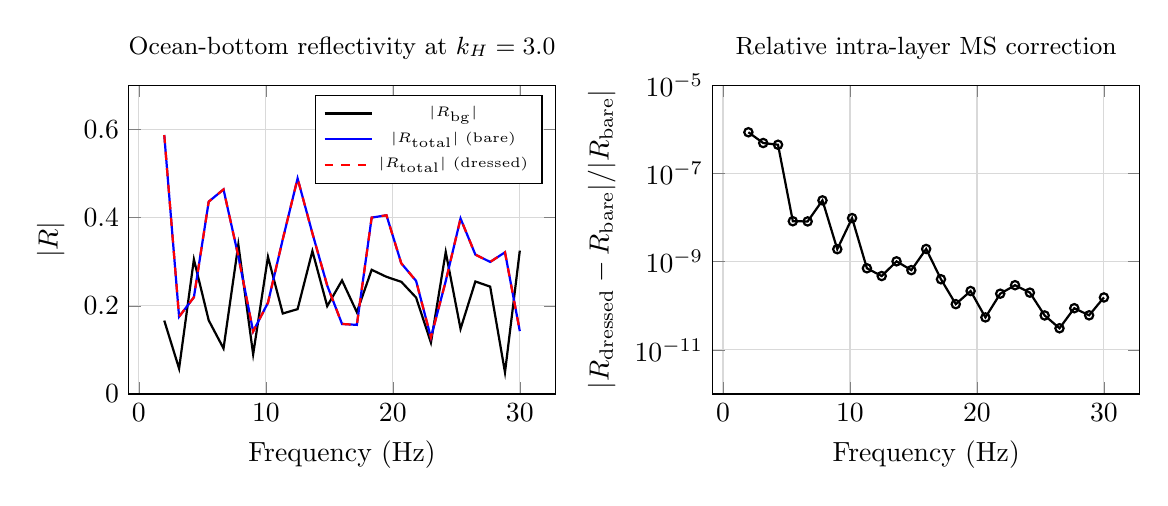
\begin{tikzpicture}
\begin{groupplot}[
  group style={
    group size=2 by 1,
    horizontal sep=2.0cm,
  },
  width=7cm, height=5.5cm,
  grid=major,
  grid style={gray!30},
]

% Left: absolute reflectivities
\nextgroupplot[
  xlabel={Frequency (Hz)},
  ylabel={$|R|$},
  title={Ocean-bottom reflectivity at $k_H = 3.0$},
  title style={font=\small},
  legend pos=north east,
  legend style={font=\tiny},
  ymin=0, ymax=0.7,
]
\addplot[black, thick, mark=none] coordinates {
  (2.000000, 0.166486)
  (3.166667, 0.057678)
  (4.333333, 0.305196)
  (5.500000, 0.167001)
  (6.666667, 0.103292)
  (7.833333, 0.339013)
  (9.000000, 0.090077)
  (10.166667, 0.311102)
  (11.333333, 0.182573)
  (12.500000, 0.192417)
  (13.666667, 0.324191)
  (14.833333, 0.199296)
  (16.000000, 0.257655)
  (17.166667, 0.185458)
  (18.333333, 0.281700)
  (19.500000, 0.265750)
  (20.666667, 0.254495)
  (21.833333, 0.218723)
  (23.000000, 0.116460)
  (24.166667, 0.321975)
  (25.333333, 0.147698)
  (26.500000, 0.255181)
  (27.666667, 0.243474)
  (28.833333, 0.049017)
  (30.000000, 0.325170)
};
\addlegendentry{$|R_{\mathrm{bg}}|$}

\addplot[blue, thick, mark=none] coordinates {
  (2.000000, 0.587443)
  (3.166667, 0.175322)
  (4.333333, 0.219362)
  (5.500000, 0.436247)
  (6.666667, 0.464008)
  (7.833333, 0.312526)
  (9.000000, 0.141815)
  (10.166667, 0.207027)
  (11.333333, 0.350948)
  (12.500000, 0.488928)
  (13.666667, 0.364567)
  (14.833333, 0.245948)
  (16.000000, 0.158793)
  (17.166667, 0.156727)
  (18.333333, 0.400133)
  (19.500000, 0.405404)
  (20.666667, 0.296364)
  (21.833333, 0.256453)
  (23.000000, 0.128080)
  (24.166667, 0.255958)
  (25.333333, 0.398078)
  (26.500000, 0.316156)
  (27.666667, 0.299522)
  (28.833333, 0.321378)
  (30.000000, 0.142613)
};
\addlegendentry{$|R_{\mathrm{total}}|$ (bare)}

\addplot[red, thick, dashed, mark=none] coordinates {
  (2.000000, 0.587443)
  (3.166667, 0.175322)
  (4.333333, 0.219362)
  (5.500000, 0.436247)
  (6.666667, 0.464008)
  (7.833333, 0.312526)
  (9.000000, 0.141815)
  (10.166667, 0.207027)
  (11.333333, 0.350948)
  (12.500000, 0.488928)
  (13.666667, 0.364567)
  (14.833333, 0.245948)
  (16.000000, 0.158793)
  (17.166667, 0.156727)
  (18.333333, 0.400133)
  (19.500000, 0.405404)
  (20.666667, 0.296364)
  (21.833333, 0.256453)
  (23.000000, 0.128080)
  (24.166667, 0.255958)
  (25.333333, 0.398078)
  (26.500000, 0.316156)
  (27.666667, 0.299522)
  (28.833333, 0.321378)
  (30.000000, 0.142613)
};
\addlegendentry{$|R_{\mathrm{total}}|$ (dressed)}

% Right: relative correction
\nextgroupplot[
  xlabel={Frequency (Hz)},
  ylabel={$|R_{\mathrm{dressed}} - R_{\mathrm{bare}}|
    / |R_{\mathrm{bare}}|$},
  title={Relative intra-layer MS correction},
  title style={font=\small},
  ymode=log,
  ymin=1e-12, ymax=1e-5,
]
\addplot[black, mark=o, mark size=1.5pt, thick] coordinates {
  (2.000000, 8.659e-07)
  (3.166667, 4.935e-07)
  (4.333333, 4.509e-07)
  (5.500000, 8.296e-09)
  (6.666667, 8.212e-09)
  (7.833333, 2.466e-08)
  (9.000000, 1.925e-09)
  (10.166667, 9.774e-09)
  (11.333333, 7.102e-10)
  (12.500000, 4.739e-10)
  (13.666667, 1.021e-09)
  (14.833333, 6.447e-10)
  (16.000000, 1.949e-09)
  (17.166667, 4.005e-10)
  (18.333333, 1.091e-10)
  (19.500000, 2.165e-10)
  (20.666667, 5.451e-11)
  (21.833333, 1.883e-10)
  (23.000000, 2.935e-10)
  (24.166667, 1.990e-10)
  (25.333333, 6.041e-11)
  (26.500000, 3.094e-11)
  (27.666667, 8.829e-11)
  (28.833333, 6.084e-11)
  (30.000000, 1.547e-10)
};

\end{groupplot}
\end{tikzpicture}
\caption{Ocean-bottom reflectivity at $k_H = 3.0$~km$^{-1}$ (hard
contrast).  \textbf{Left:} the background reflectivity $|R_{\mathrm{bg}}|$
(black) and total reflectivity with scatterers (blue = bare,
red dashed = dressed); bare and dressed curves coincide exactly.
\textbf{Right:} the relative difference between dressed and bare total
reflectivities is at the level of numerical precision
($10^{-7}$--$10^{-11}$).}
\label{fig:reflectivity}
\end{figure}

Two features are noteworthy:

\begin{enumerate}[nosep]
\item \textbf{Scattering is significant.}  The total reflectivity
  (blue/red) differs markedly from the background (black), confirming
  that the interlayer Foldy-Lax solver produces a non-trivial scattering
  correction at the ocean bottom.

\item \textbf{Bare and dressed T yield identical reflectivity.}
  Despite the 275\% correction to the individual T-matrix norm, the
  ocean-bottom reflectivity is insensitive to the bare-vs-dressed
  distinction.  The relative difference (right panel) is at the level
  of floating-point precision ($< 10^{-7}$).
\end{enumerate}

The insensitivity arises because the interlayer Foldy-Lax system
operates in a strong multiple scattering regime: the Foldy-Lax
exciting field $\bm{\psi}_{\mathrm{exc}}$ is approximately $10^{14}$
times smaller than the incident field $\bm{\psi}_{\mathrm{inc}}$,
indicating that the matrix $(\mathbf{I} - \mathbf{G} \cdot \mathbf{T})$
nearly annihilates the incident field.  In this regime, the system
self-regulates: the exciting field adjusts to compensate for changes in
$\mathbf{T}$, producing the same scattered reflectivity regardless of
whether the bare or dressed T-matrix is used.  The Born approximation
(which replaces $\bm{\psi}_{\mathrm{exc}}$ with
$\bm{\psi}_{\mathrm{inc}}$) grossly overestimates the scattering by a
factor of ${\sim}10^{13}$, confirming that multiple scattering
dominates.

\begin{remark}
This result does not diminish the physical significance of the dressed
T-matrix.  For an effective-medium description of a single horizontal
layer --- where the Riccati interlayer solver treats each interface as a
homogenised scattering plane --- the dressed T correctly captures the
intra-layer self-energy.  The insensitivity observed here is specific to
the interlayer Foldy-Lax formulation with two closely spaced scatterer
interfaces, where the strong vertical coupling dominates.
\end{remark}

%=============================================================================
\section{Conclusions}\label{sec:conclusions}
%=============================================================================

Three key results emerge from this study:

\begin{enumerate}
\item \textbf{Solver correctness.}  The block-preconditioned Foldy-Lax
  solver, using 2D FFT convolution per z-layer pair and an outer GMRES,
  matches the dense reference solve to relative errors below
  $3.35 \times 10^{-7}$ across all tested configurations
  ($M \in \{3, 5\}$, $N_z \in \{1, 2, 3\}$).

\item \textbf{Interlayer coupling.}  The per-cube composite T-matrix
  norm grows monotonically with slab thickness $N_z$, increasing by a
  factor of 2.2 from $N_z = 1$ to $N_z = 5$.  This quantifies the
  interlayer vertical multiple scattering that a single-layer
  description misses.

\item \textbf{Reflectivity saturation.}  In the interlayer Foldy-Lax
  solver for ocean-bottom reflectivity, bare and dressed T-matrices
  produce identical results despite a 275\% correction to the individual
  T-matrix.  This saturation effect arises from strong multiple
  scattering between scatterer interfaces: the Foldy-Lax exciting
  field self-regulates, absorbing the T-matrix correction into a
  compensating change in $\bm{\psi}_{\mathrm{exc}}$.
\end{enumerate}

%=============================================================================
\section*{References}
%=============================================================================

\begin{enumerate}[label={[\arabic*]},nosep]
  \item L.L.\ Foldy, ``The multiple scattering of waves.\ I.\ General
    theory of isotropic scattering by randomly distributed scatterers,''
    \emph{Phys.\ Rev.}, vol.~67, pp.~107--119, 1945.
  \item M.\ Lax, ``Multiple scattering of waves.\ II.\ The effective
    field in dense systems,'' \emph{Phys.\ Rev.}, vol.~85,
    pp.~621--629, 1952.
  \item B.L.N.\ Kennett, \emph{Seismic Wave Propagation in Stratified
    Media}, Cambridge University Press, 1983.
  \item P.A.\ Martin, \emph{Multiple Scattering: Interaction of
    Time-Harmonic Waves with $N$ Obstacles}, Cambridge University
    Press, 2006.
  \item Y.\ Saad and M.H.\ Schultz, ``GMRES: A generalized minimal
    residual algorithm for solving nonsymmetric linear systems,''
    \emph{SIAM J.\ Sci.\ Stat.\ Comput.}, vol.~7, pp.~856--869, 1986.
  \item T.M.\ Nestor, \emph{Elastic Multiple Scattering from
    Heterogeneities in Layered Marine Sediments}, PhD thesis,
    University of Sydney, 1996.
\end{enumerate}

\end{document}
